%----------------------------------------------------------
\chapter{Классификация систем типов}
\label{ch:classification}
%----------------------------------------------------------

Известно, что системы типов можно разделить на \textit{динамические} и \textit{статические} \cite{Typing}.
Это влияет на то, в какой момент в программе происходит проверка соответствия типов.
В динамических системах - во время исполнения программы, а в статических - соответственно во время компиляции.
Кроме того, существуют особые языки программирования, где все данные имеют один тип.
К таким относятся многие низкоуровневые языки, например ассемблер.
Все данные в нем (адреса в памяти, числа, указатели на функции) являются всего лишь последовательностью байт.

Ниже приведены основные критерии, по которым можно классифицировать систему типов в языках программирования:

\begin{enumerate}[1)]
    \item по времени проверки соответствия типам: статическая и динамическая,
    \item по поддержке неявных конверсий: сильная (англ. strong) и слабая,
    \item по необходимости вручную типизировать выражение: явная и неявная.
\end{enumerate}

Например, типизация в язык python является динамической, сильной и неявной с точки зрения этой классификации \cite{PythonWiki}.
Интерпретатор знает тип переменной только во время выполнения и не может неявно изменить его.

Далее будут рассмотрены только статические системы типов, так как после семантического анализа, компилятор может использовать накопленную информацию для оптимизации кода.
Это делает языки со статической типизацией, хоть и более сложными в использовании, но более быстрыми, а динамически типизированным языкам приходится использовать различные специфические оптимизации, например, \textit{JIT-компиляцию}, чтобы добиться сопоставимой скорости.

JIT-компиляцией называется прием оптимизации выполнения, когда компиляция происходит и во время работы программы.
Благодаря этому можно оптимизировать некоторые особые случаи.

Предлагается исследовать существующие решения среди различных языков программирования и выделить в них положительные и отрицательные стороны.

\section{Система типов C}
\label{sec:c_type_system}

C - язык программирования со статической, слабой, явной типизацией, разработанный в 1970-х годах.

Типом в языке C является интерпретация набора байт, составляющих объект \cite{CSpec}.
Все типы делятся на две группы: скалярные и агрегатные (рис. \ref{fig:c_types}).
К скалярным типам относят примитивные (базовые) типы, которые описывают множество различных вариантов представления числа, а также указатели.
К агрегатным - определяемые пользователем структуры, состоящие из упорядоченного именованного набора других типов, и массивы какого-то конкретного типа.

Кроме того, существуют <<специальные>> типы - объединения и функции.
Специальные они потому что в первом случае - это лишь особый вариант структуры, а во втором - существуют только указатели на функции: отдельного типа для \textit{лямбда-функции} в C нет.

Лямбда-функцией в информатике называют анонимную функцию.

\begin{figure}[H]
    \centering
    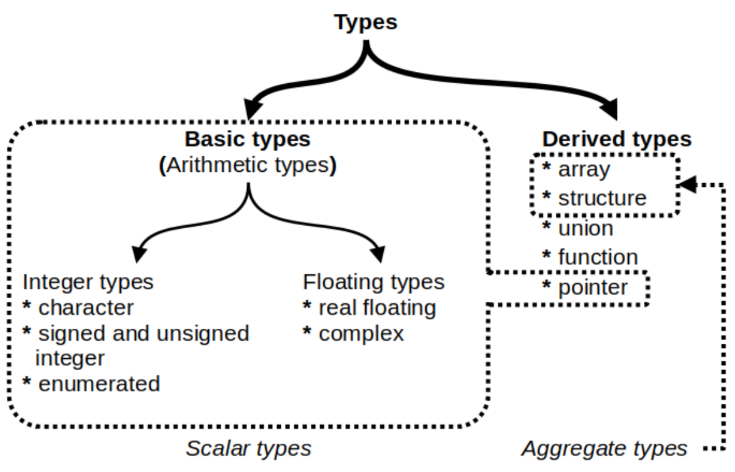
\includegraphics[width=0.9\textwidth]{figures/c_types}
    \caption{Схематичное изображение типов в C}
    \label{fig:c_types}
\end{figure}

Достоинства:
\begin{itemize}
    \item C прост для понимания, он содержит только основные типы данных,
    \item язык позволяет эффективно работать с данными в том виде, как они реализованы в ЭВМ.
\end{itemize}

Недостатки:
\begin{itemize}
    \item недостаточная выразительность по сравнению с другими языками программирования,
    \item мало гарантий и проверок, осуществляемых компилятором.
\end{itemize}

Здесь под выразительностью стоит понимать то, насколько много идей можно реализовать и насколько лаконично они при этом будут выглядеть.
Например, хоть в C и можно выразить идею объекто-ориентированного программирования, но это будет выглядеть гораздо более громоздко, чем в C++.

\section{Система типов Kotlin}
\label{sec:kotlin_type_system}

Язык Kotlin разрабатывается компанией JetBrains с 2011 года.
Основной платформой, на которой он исполняется, является java virtual machine (JVM).
Популярен среди разработчиков приложений под ОС Android\cite{KotlinTypeSpec} из-за лаконичного синтаксиса.

Достоинства:
\begin{itemize}
    \item имеет более продвинутую, по сравнению с Java, систему типов, включающую \textit{nullable types} и ограниченно типы-произведения,
    \item в нем можно использовать все библиотеки, разработанные под JVM
\end{itemize}

Недостатки:
\begin{itemize}
    \item из-за специфики работы обобщенных типов в JVM иногда сложно узнать, какой тип у объекта во время исполнения
    \item все еще менее выразительна, по сравнению с некоторыми функциональными языками
\end{itemize}

\section{Система типов ML-подобных языков}
\label{sec:ml_type_system}

К семейству ML-подобных языков относят функциональные языки с развитой системой типов.
В основе неё лежит типизированное лямбда-исчисление.
Это формализованная система для описания программ, предложенная Алонзо Чёрчем в 1930 году и в отличие от обычного лямбда-исчисления, здесь каждому терму сопоставлен тип.

Кроме проверки типов, над такими системами можно удобно проводить \textit{вывод типов}.
Это позволяет пользователю составлять программы почти не используя аннотации типов.

Алгоритмы вывода типов позволяют компилятору узнать тип терма из контекста.

\subsection{Лямбда-куб}
\label{subsec:lambda_cube}

Эта абстракция позволяет наглядно увидеть разницу и взаимоотношение между различными видами тизипированными лямбда-исчислениями (рис. \ref{fig:lambda_cube}).

\begin{figure}[H]
    \centering
    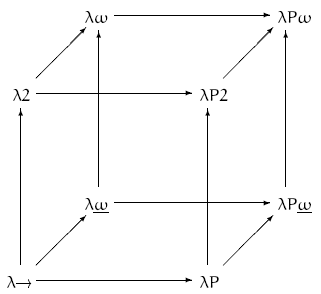
\includegraphics[width=0.55\textwidth]{figures/Lambda_cube}
    \caption{Графическое изображение лямбда-куба}
    \label{fig:lambda_cube}
\end{figure}

Простейшим вариантом является \textit{просто типизированное лямбда-исчисление} ($\lambda \to$).
В нем доступна абстракция только с помощью функции:

\begin{equation}
    \label{eq:STLC}
    \frac{\Gamma \cup x: T \vdash y: U}{\Gamma \vdash \lambda x.y: T \to U}
\end{equation}

Следующим этапом является \textit{полиморфное лямбда-исчисление} ($\lambda 2$).
В нём термы могут зависеть от типов (обобщенные функции):

\begin{equation}
    \label{eq:2TLC}
    \frac{\Gamma \vdash y: U}{\Gamma \vdash \forall T: \lambda (x: T).y: T \to U}
\end{equation}

Еще одним расширением будет \textit{лямбда-исчисление с операторами над типами} ($\lambda \underline{w}$).
С точки зрения обычных языков программирования такое исчисление формирует функции над типами:
В частности, функция, формирующая тип списка, выглядела бы так:

\begin{equation}
    \label{eq:WTLC}
    \lambda \alpha: *. \alpha \to List ~\alpha
\end{equation}, где $*$ - любой другой тип

Последней простой точкой куба является \textit{лямбда-исчисление с зависимыми типами} ($\lambda P$).
Оно примечательно тем, что типы могут зависеть от термов.
Наиболее простым примером послужит функция деления, где входной аргумент обязан быть отличным от $0$.

Остальные вершины являются комбинацией описанных систем.

Подведем итог.

Достоинства:
\begin{itemize}
    \item выразительность системы типов легко показать том же самом лямбда-кубе,
    \item имеет строгое математическое обоснование и хорошо изучено,
    \item компилятор имеет возможность выявить больше ошибок в программе.
\end{itemize}

Недостатки:
\begin{itemize}
    \item достаточно сложна для понимания как с точки зрения пользователя, так и разработчика компилятора
    \item может значительно увеличить время компиляции из-за обилия сложных алгоритмов
\end{itemize}

%----------------------------------------------------------
